\chapter{Geometry reconstruction by lookup table}\label{ch:lookupTable}

\vspace{-1.5 em}
\begin{addmargin}[-0.5cm]{0cm}
  \minitoc
\end{addmargin}
\hrule
\vspace{1.5 em}

\noindent
We begin our attempts at reconstructing geometries by taking a very simple approach, the use of a lookup table. Simulating Coulomb explosions is computationally cheap, or fast, so we can simulate the explosion of many geometries and create a large mapping of geometries to asymptotic momentum vectors. Then reconstructing a geometry from measured momentum vectors is simply a matter of looking up the geometry that produces the most similar momentum vector arrangement. In this chapter we will describe an implementation of this approach and use it to reconstruct molecular geometries for carbonyl sulfide (\ch{OCS}) in the \ch{OCS $\rightarrow$ O^{2+} + C^{2+} + S^{2+}} concerted\footnotemark~ fragmentation channel, denoted as the $(2,2,2)$ channel.

\footnotetext{Meaning that the molecule dissociates into its atomic fragments at the beginning of the Coulomb explosion, simplifying the system's dynamics and simulation. This is opposed to, for example, stepwise dissociation in which the two bonds break at different times, allowing for the formation of a diatomic rotor, or dumbbell, which rotates numerous times before further dissociating into its atomic fragments.}

% Following the implementation details, we will discuss some of the drawbacks of using a lookup table which we will see are severe enough to warrant the immediate search for another method, laying the motivation for the next chapter. The lookup table will also lead us to some new insights regarding the geometry reconstruction problem in general, alerting us specifically to the existence of \emph{degenerate geometries}. However, before fully abandoning this approach, we will also discuss its usefulness in future applications.

First doing so however, we will motivate the need for a new approach to geometry reconstruction, the lookup table, by investigating the failures of the previous attempt at reconstructing molecular geometries, which relied on the Nelder-Mead simplex method. We will also take a brief historical look at lookup tables.

\section{Previous attempt using the Nelder-Mead method} \label{sec:nelderMead}
\index{Simplex algorithm}
\index{Geometry reconstruction!Simplex algorithm}
\citet{Brichta09} proposed the reconstruction of small triatomic molecules using a ``simplex'' algorithm. It should not be confused with the much better known simplex algorithm by George Dantzig, also an optimization algorithm but for linear programming (see section \ref{ssec:elementaryOptimization}). The algorithm employed should be referred to as the Nelder-Mead method, downhill simplex method, or amoeba method to avoid confusion between the two.\footnotemark~ We refer to it as the \emph{Nelder-Mead method} for this chapter, as Wikipedia does.

\footnotetext{It seems that Dantzig's simplex algorithm finds more use in fields such as optimization, operations research, and economics while the Nelder-Mead simplex method has been historically popular in scientific and engineering fields due to it's ability to run on microcomputers.}

\subsection{Previous reconstructions}
Unfortunately, \citet{Brichta09} only report on the reconstruction of molecular structures based on a few simulated geometries for carbon dioxide (\ch{CO2}) and formaldehyde (\ch{CH2O}). In an earlier work, \citet{Brichta07} used this algorithm to report on reconstructions of \ch{CO2} geometries from experimental data (see figure \ref{fig:simplexJPhysB}), which seems ripe for discussion and investigation, however the experimental data is not discussed and instead the focus is placed on reconstructing simulated data. They plot the ground state geometry of \ch{CO2} as perfectly linear even though it should have a bond angle of \SI{172.5}{\degree} \citep{Siegmann02, Mathur92}. Each plot is reported to contain approximately $10^3$ events (or geometries), however figures \ref{fig:simplexJPhysB}(a) and (d) appear to contain quite different amounts of data. It was also used by \citet{Bocharova11} to report on the molecular structure of \ch{CO2} $(2,2,2)$ (see figure \ref{fig:simplexPRL}). They report a molecular geometry of $\langle r_\mathrm{CO} \rangle \approx \SI{1.3}{\angstrom}$, $\langle \theta_\mathrm{OCO} \rangle \approx 168\degree$ which is close the equilibrium geometry of $\langle r_\mathrm{CO} \rangle \approx \SI{1.16}{\angstrom}$ \citep{ChemistryOfTheElements} and $\langle \theta_\mathrm{OCO} \rangle \approx \SI{172}{\degree}$ \citep{Siegmann02, Mathur92}.

\begin{figure}
  \centering
  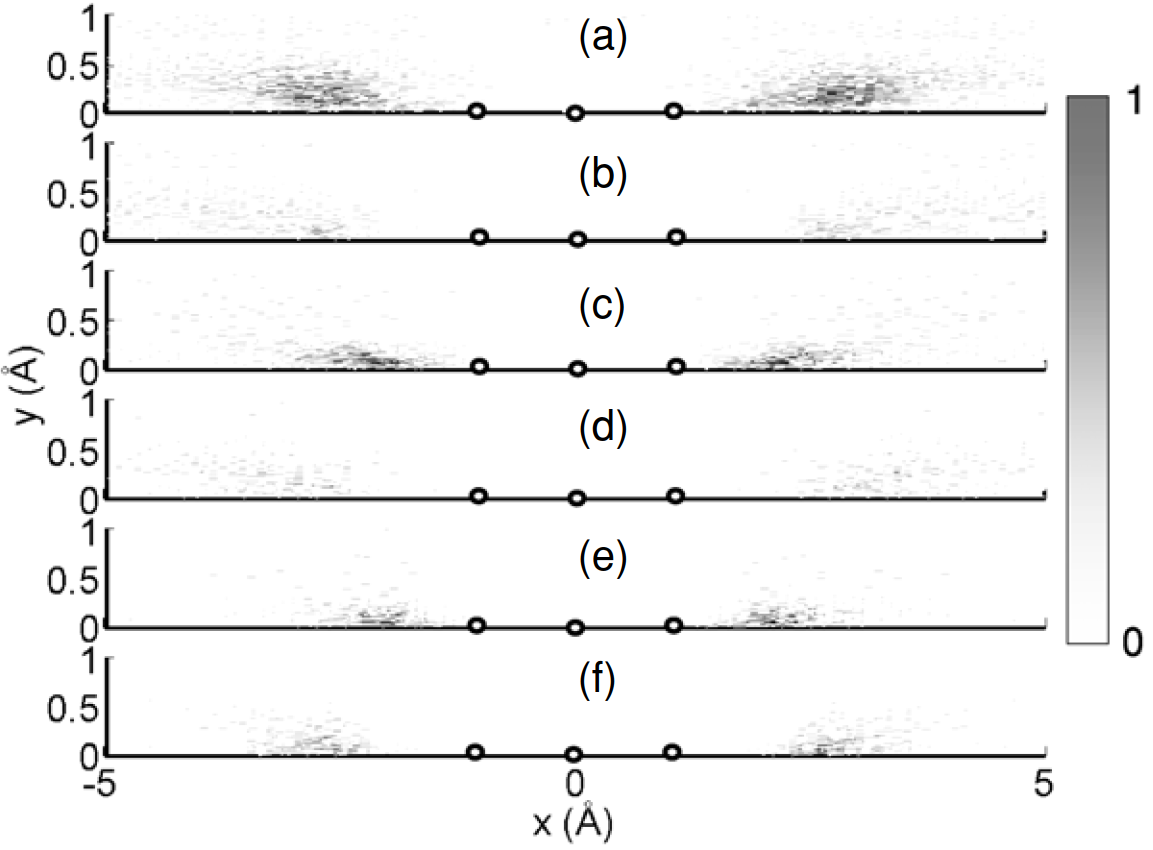
\includegraphics[width=\textwidth]{gfx/SimplexJPhysB}
  \caption[Reconstructed \ch{CO2} geometries using the Nelder-Mead simplex method.]
  {Reconstructed \ch{CO2} geometries after Coulomb explosion by \SI{50}{\fs} laser pulses using the Nelder-Mead simplex method for the (a) $(1,1,1)$, (b) $(1,2,1)$, (c) $(1,1,2)$, (d) $(1,2,2)$, (e) $(2,1,2)$, and (f) $(2,2,2)$ fragmentation channels. The carbon atom is placed at the origin with the higher charged oxygen atom in the +$x$-quadrant. A $2$D histogram is used to plot the spatial distribution of the two terminal oxygen atoms with darker colors indicating a higher count rate. The histogram is normalized such that the maximum count rate is $1$. The three circles represent the equilibrium or ground state geometry of \ch{CO2}. Figure from \citet{Brichta07}.}
  \label{fig:simplexJPhysB}
\end{figure}

\begin{figure}
  \centering
  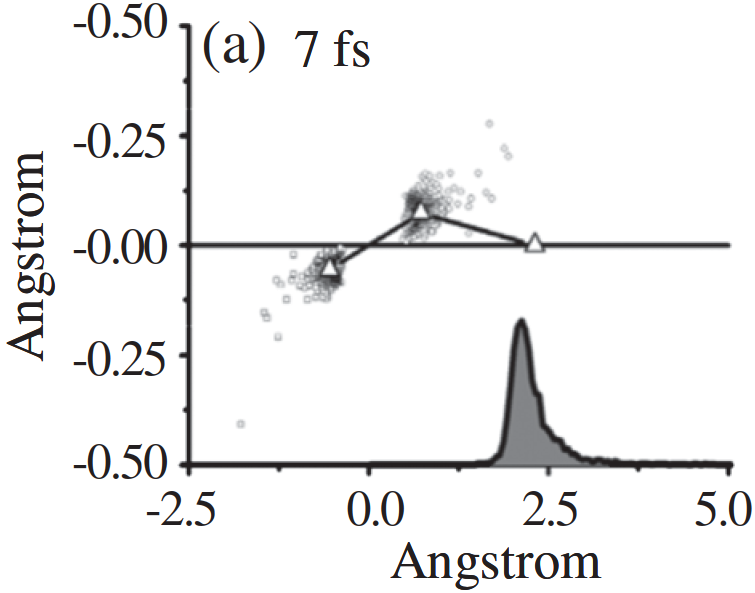
\includegraphics[width=0.6\textwidth]{gfx/SimplexPRL}
  \caption[Reconstructed \ch{CO2} in the $(2,2,2)$ charge state using the Nelder-Mead simplex method.]
  {Reconstructed \ch{CO2} geometries in the $(2,2,2)$ charge state after explosion by a \SI{7}{\fs} laser pulse using the Nelder-Mead simplex method. The oxygen in the $x>0$ plane is restricted to the $x$-axis with a probability density curve showing its distribution in space, presumably calculated using a kernel density estimate, although unreported. The circles pinpoint the location of the carbon atom and the oxygen atom in the $x<0$ plane relative to the fixed oxygen atom and the triangles presumably pinpoint the centroid (or average) position of each atom. Figure from \citet{Bocharova11}.}
  \label{fig:simplexPRL}
\end{figure}

They both produce nice and intuitive plots, showing what appears to be an approximation to a molecular wavefunction with two broad position distributions as one atom is fixed. Both works, however, do not report the set of geometries used to form the initial simplex.

\subsection{Testing the Nelder-Mead method} \label{ssec:simplexFail}
% TODO: Move this somewhere?
% When we initially attempted to apply the Nelder-Mead simplex method to the problem of geometry reconstruction ourselves, we found the results to vary greatly depending on the set of geometries chosen to form the initial simplex, required by the algorithm as an input parameter, similar to an initial guess. The majority of reconstructed geometries did not make physical sense, such as reconstructing one bond length which was several times an order-of-magnitude longer than the other.

Before using the Nelder-Mead to reconstruct geometries besides \ch{CO2}, such as \ch{OCS}, we decided to investigate the accuracy and reliability of the Nelder-Mead method for geometry reconstruction, by testing to see whether it could reconstruct simulated geometries. By this we mean that we would chose a molecular geometry then use it to simulate a Coulomb explosion (see section \ref{sec:simulating}) and compute the resulting asymptotic momentum vectors. These momentum vectors are then fed into the Nelder-Mead method to see whether it could recover the original molecular geometry, as done by \citet{Brichta09}.

\subsubsection*{Methodology: attempting to reconstruct simulated geometries}
Simulated geometries are used for this analysis because we can check exactly how far off the reconstructed geometry is from the known correct solution. The simulated geometry only experiences the Coulomb force and so at least one solution is guaranteed to exist by our deterministic classical simulation. Simulated geometries are thus the easiest geometries to reconstruct and serious doubts regarding an algorithm's utility must be raised if it cannot reconstruct them. When dealing with experimentally measured data, we do not know the geometries \textit{a priori} and so we need a trustworthy reconstruction algorithm in order to trust any of the results it produces.

% What we found confirmed the unreliable nature of the Nelder-Mead method for reconstructing molecular geometries.

We attempted to reconstruct molecular structures for \ch{CO2} and \ch{OCS}, both in the $(2,2,2)$ fragmentation channel. Starting from their equilibrium geometries we varied one parameter at a time to test whether the Nelder-Mead method could recover the geometry. The initial simplex we used for reconstructing \ch{CO2} and \ch{OCS} consist of four points (or initial guess geometries) and are tabulated in table \ref{table:initialSimplex}.

\begin{table}
  \myfloatalign
  \centering
  \begin{tabularx}{0.85\textwidth}{cccccc}
    \toprule
    \multicolumn{3}{c}{\ch{CO2} simplex} & \multicolumn{3}{c}{\ch{OCS} simplex} \\
    $r_\mathrm{12}$ (\SI{}{\angstrom}) & $r_\mathrm{23}$ (\SI{}{\angstrom}) & $\theta_\mathrm{OCO}$ (\SI{}{\degree}) & $r_\mathrm{CO}$ (\SI{}{\angstrom}) & $r_\mathrm{CS}$ (\SI{}{\angstrom}) & $\theta_\mathrm{OCS}$ (\SI{}{\degree}) \\
    \midrule
    0.9 & 1.2 & 165 & 1.8 & 2.4 & 165 \\
    1.4 & 1.0 & 165 & 0.8 & 1.5 & 165 \\
    0.9 & 1.9 & 165 & 1.8 & 3.8 & 165 \\
    0.9 & 1.2 & 180 & 1.8 & 2.4 & 180 \\
    \bottomrule
  \end{tabularx}
  \caption[Initial \ch{CO2} and \ch{OCS} simplices used for testing the Nelder-Mead method.]
  {Initial \ch{CO2} and \ch{OCS} simplices used for testing the Nelder-Mead method.}
  \label{table:initialSimplex}
\end{table}

\subsubsection*{Results}
Figure \ref{fig:CO2SimplexCalibrationPlots} shows the reconstruction results for \ch{CO2} $(2,2,2)$. We take the ground state geometry of \ch{CO2} to be $r_\mathrm{CO} = \SI{1.16}{\angstrom}$ \citep{ChemistryOfTheElements} and $\theta_\mathrm{OCO} = \SI{180}{\degree}$ although $\theta_\mathrm{OCO} = \SI{172}{\degree}$ would be more accurate \citep{Siegmann02, Mathur92}.

\begin{figure}
  \centering
  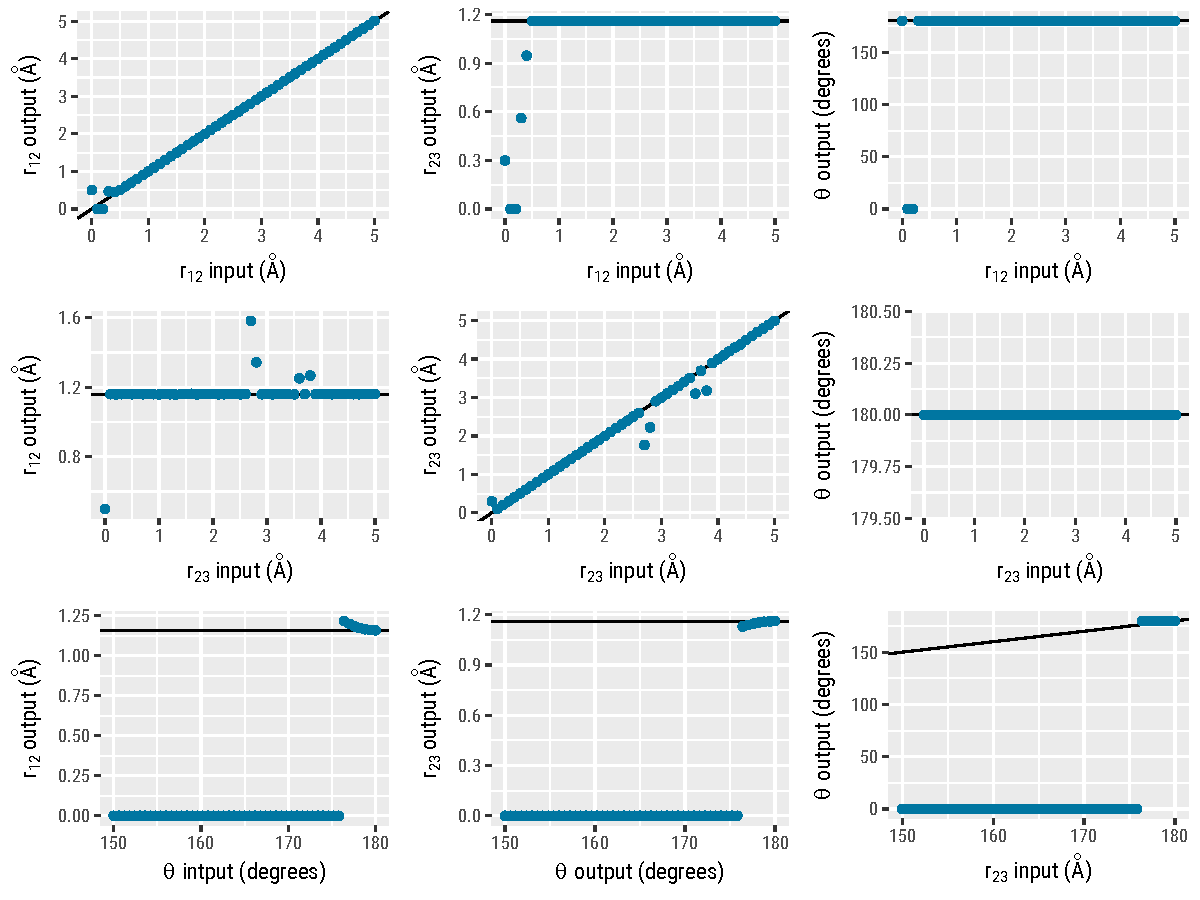
\includegraphics[width=\textwidth]{Plots/CO2SimplexCalibrationPlots}
  \caption[Testing the Nelder-Mead method's ability to reconstruct \ch{CO2} (2,2,2) geometries]
  {Testing the Nelder-Mead method's ability to reconstruct \ch{CO2} geometries in the (2,2,2) fragmentation channel by starting with the ground-state geometry of \ch{CO2} and varying each parameter one-by-one. Solid black lines indicate the expected output geometry.}
  \label{fig:CO2SimplexCalibrationPlots}
\end{figure}

In the first row of figure \ref{fig:CO2SimplexCalibrationPlots}, the first \ch{C-O} bond length ($r_{12}$) was varied to create an ``input geometry'' which underwent a simulated Coulomb explosion. The resulting momentum vectors from the explosion were fed into the Nelder-Mead method which converged to a geometry we call the reconstructed or ``output'' geometry. The second \ch{C-O} bond length ($r_{23}$) and the bond angle $\theta$ were varied in the second and third rows respectively. Solid black lines indicate the expected output geometry, so deviations indicate a failure on the method's ability to reconstruct the geometry. We see that the algorithm can accurately reconstruct the geometry when a single bond length is varied but completely fails once the bond angle is below approximately $176\degree$, at which point the reconstruction code was instructed to simply return a row of zeros, thus the large number of data points with output bond lengths and angles of zero in the third row.

Figure \ref{fig:OCSSimplexCalibrationPlots} shows the reconstruction results for \ch{OCS} $(2,2,2)$. For \ch{OCS}, we took the ground state geometry to be $r_\mathrm{CO} = \SI{1.1578}{\angstrom}$, $r_\mathrm{CS} = \SI{1.5601}{\angstrom}$ \citep{CRCHandbook88ed}, and $\theta_\mathrm{OCS} = \SI{180}{\degree}$ although $\theta_\mathrm{OCS} = \SI{175}{\degree}$ \citep{Wales12HCI} would be more accurate \citep{Wales12HCI}.

\begin{figure}
  \centering
  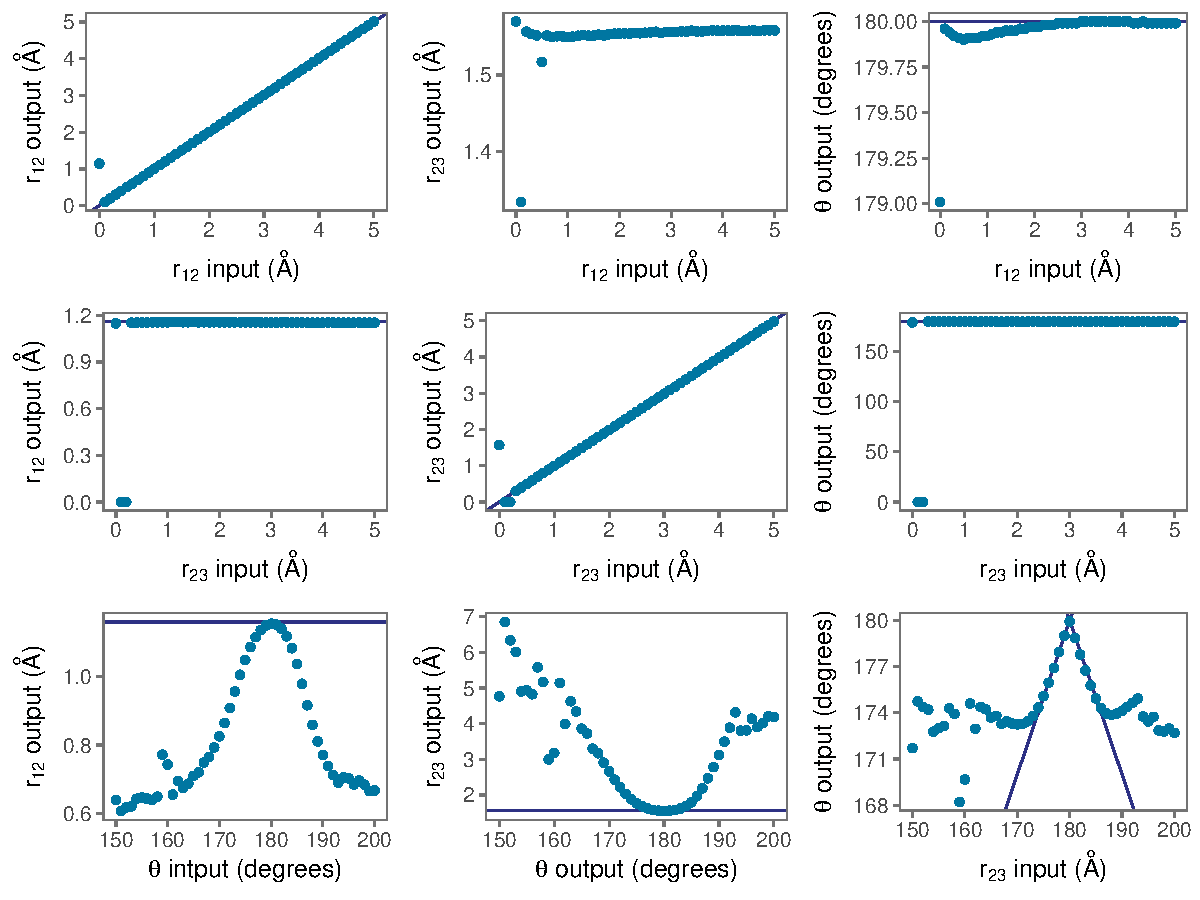
\includegraphics[width=\textwidth]{Plots/OCSSimplexCalibrationPlots}
  \caption[Testing the Nelder-Mead method's ability to reconstruct \ch{OCS} (2,2,2) geometries.]
  {Testing the Nelder-Mead method's ability to reconstruct \ch{OCS} (2,2,2) geometries by starting with the ground-state geometry of \ch{OCS} and varying each parameter one-by-one. Solid black lines indicate the expected output geometry.}
  \label{fig:OCSSimplexCalibrationPlots}
\end{figure}

In the first row of figure \ref{fig:OCSSimplexCalibrationPlots}, the \ch{C-O} bond length ($r_\textrm{CO}\equiv r_{12}$) was varied to create an ``input geometry'' which underwent a simulated Coulomb explosion. The resulting momentum vectors from the explosion were fed into the Nelder-Mead algorithm which converged to a geometry, the ``output geometry''. The \ch{C-S} bond length ($r_\textrm{CS}\equiv r_{23}$) and the bond angle $\theta$ were varied in the second and third rows respectively. A triatomic molecule with a bond angle greater than \SI{180}{\degree}, $\SI{180}{\degree} + x\degree$ for example, is the same as a molecule with a bond angle of $\SI{180}{\degree} - x\degree$, and so it should not be necessary to attempt the reconstruction of geometries with bond angles greater than \SI{180}{\degree} but we attempt it nonetheless with the aim of testing the method's robustness. Solid black lines indicate the expected output geometry, so deviations indicate a failure on the algorithm's ability to reconstruct the geometry. We see that the algorithm can accurately reconstruct the geometry when a single bond length is varied but performs worse and worse as the molecule bends, even slightly. There are some slight differences between molecules with bond angles of $\SI{180}{\degree} + x\degree$ and $\SI{180}{\degree} - x\degree$, but the absolute errors on the reconstructed bond lengths and angles seems to be similar for both cases.

\subsubsection*{Discussion}
So we see that the Nelder-Mead method successfully retrieves the bond lengths for the majority of cases but not the bond angles. In the case of \ch{CO2} it seems to completely fail at retrieving the geometry once the bond angle falls below approximately $176\degree$. For \ch{OCS}, the absolute error on the reconstructed bond angle seems to increase quadratically as the molecule bends, even slightly.

A more thorough analysis should vary multiple parameters at once to more fully explore the state space of the problem, however if the method cannot even reconstruct geometries that slightly different from the equilibrium state by a single parameter as we have done, then the results of a more thorough analysis will probably be even more worrying.

It should be noted that the Nelder-Mead method is quite sensitive to the geometries chosen to represent the initial simplex. Changing them could significantly impact the algorithm's ability to converge on the correct geometry. Of course, this does suggest that there may exist a set of initial geometries that significantly improve the algorithm's reliability, however, I could not find such a set even after several dozen attempts. Some choices improved the recovery of bond angles at the cost of failing to recover the correct bond lengths. The initial simplex used to produce figures \ref{fig:CO2SimplexCalibrationPlots} and \ref{fig:OCSSimplexCalibrationPlots} was chosen to maximize the number of successful reconstructions for very straight molecules which constitute the majority of cases, however molecules with bond angles $\theta < 175\degree$ are still very common and so even with this choice, we are very unsure about the accuracy of the majority of reconstructions.

The Nelder-Mead algorithm is an ad-hoc or heuristic algorithm for nonlinear optimization that can be used without computing derivatives of the objective function\footnotemark. It was first generalized to minimizing functions by \citet{Nelder65} based off ideas by \citet{Spendley62}. Nelder and Mead were researchers at the National Vegetable Research Station in Warwick, England, leading an unidentified laboratory to doubt if these ``turnip bashers could be numerate'' in response to their optimization algorithm \citep{Wright10}. It has enjoyed widespread popularity due to its ease of implementation and intuitive inner workings but it is not appropriate to every problem. In fact, it is not guaranteed to converge except for strictly convex problems in 1 and 2-dimensions \citep{Lagarias98} and thus fails when applied to some problems. It can even converge to non-stationary points in some cases \citep{McKinnon98}. Studies would sometimes introduce modifications to the Nelder-Mead method that would improve its performance on a specific problem \citet{Wright10}. Unfortunately, I believe geometry reconstruction is not an appropriate problem for the Nelder-Mead method.

\footnotetext{\citet{Wright10} provides a great discussion of the Nelder-Mead method, ending with a comment by John Nelder regarding his algorithm, ``Mathematicians hate it because you can’t prove convergence; engineers seem to love it because it often works.'' \citet[section 10.4]{NumericalRecipes} describes the algorithm in detail and provides a well-commented C++ implementation.}

\subsubsection*{Conclusion}
Perhaps \citet{Brichta07} and \citet{Bocharova11} happened to find an optimal set of geometries to form their initial simplex used to produce figures \ref{fig:simplexJPhysB} and \ref{fig:simplexPRL}, however no mention of it is made anywhere, and thus we are unable to replicate their results or use the Nelder-Mead method for further reconstructions. The necessity and difficulty of fine tuning required should cast some doubt over their geometry reconstructions and any consequent conclusions in their respective works. We already have enough information to distrust the Nelder-Mead method and begin searching for a new approach.

\section{An aside on lookup tables}
The idea of using a lookup table to speed up calculations is as old as mathematics itself with examples dating back to some of the earliest mathematical texts produced by ancient Egyptian scribes during the Twelfth Dynasty of Egypt (circa 1990--1800 BC) \citep[p. 1, footnote 4]{Neugebauer45}. The Egyptian Mathematical Leather Roll, a particularly well-preserved example of Egyptian mathematics dating back to circa $1650$ BC, contains perhaps the first such complete lookup table and tabulates 26 sums of unit fractions equaling another unit fraction. \citet{Glanville27} reports on the leather roll, housed at the British Museum, and gives a photograph (figure \ref{fig:EMLR}) and schematic (figure \ref{fig:EMLRschematic}) of the table. 

% The most familiar lookup table may be the multiplication times table that every elementary school student is familiar where sets of two integers are mapped to their product. Lookup tables have been employed since antiquity and one of the earliest surviving examples is a 98-column multiplication table from 493 A.D. attributed to the Roman, Victorius of Aquitaine \citep{Maher01}. Before the advent of the calculator and for much of scientific history, extensive logarithm tables were used to look up their values to several decimal places and to speed up computations. The earliest such tables date back to the ancient greeks although they have since been lost, and the earliest surviving one is a sine table by the ancient Indian mathematician \={A}ryabha\d{t}a circa 499 C.E. \citep{Hayashi97}.

\begin{figure}
  \centering
  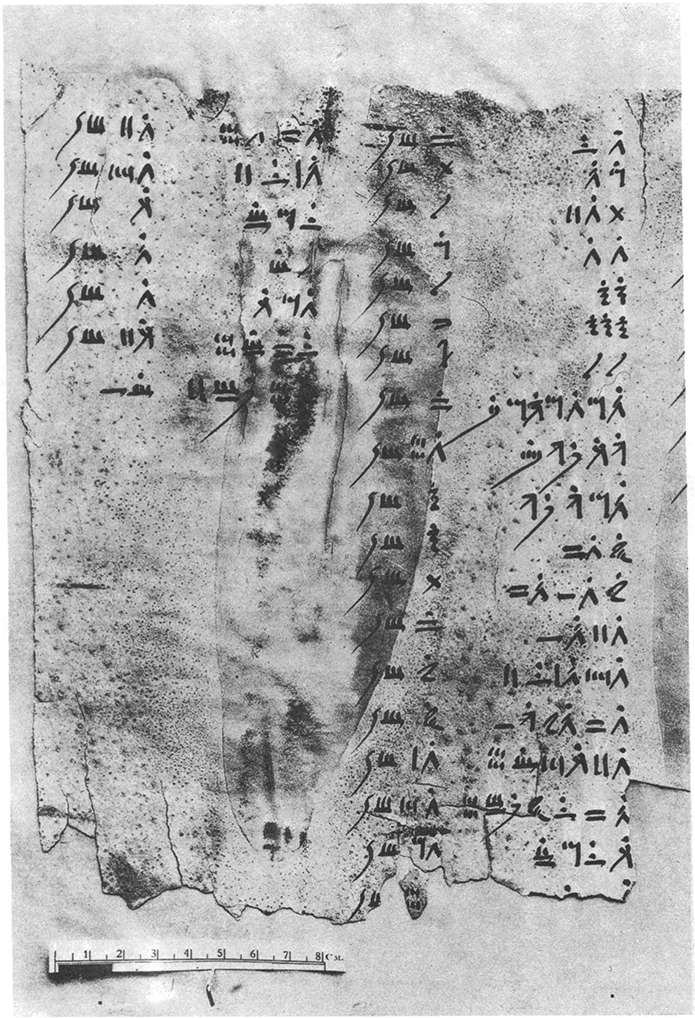
\includegraphics[width=\textwidth]{gfx/EMLR}
  \caption[Photograph of columns 3 and 4 of the Egyptian Mathematical Leather Roll.]
  {Photograph of columns 3 (right) and 4 (left) of the Egyptian Mathematical Leather Roll. Columns 3 and 4 are duplicates of columns 1 and 2. For example, row 9 of column 3 translates to $\displaystyle \frac{1}{50}\frac{1}{30}\frac{1}{150}\frac{1}{400} \quad\quad \frac{1}{16}$ in modern fraction notation where addition is implied. Figure \ref{fig:EMLRschematic} is a schematic of the table photographed here. Figure from \citet{Glanville27} which is accompanied by a translation of the hieroglyphics.}
  \label{fig:EMLR}
\end{figure}

\begin{figure}
  \centering
  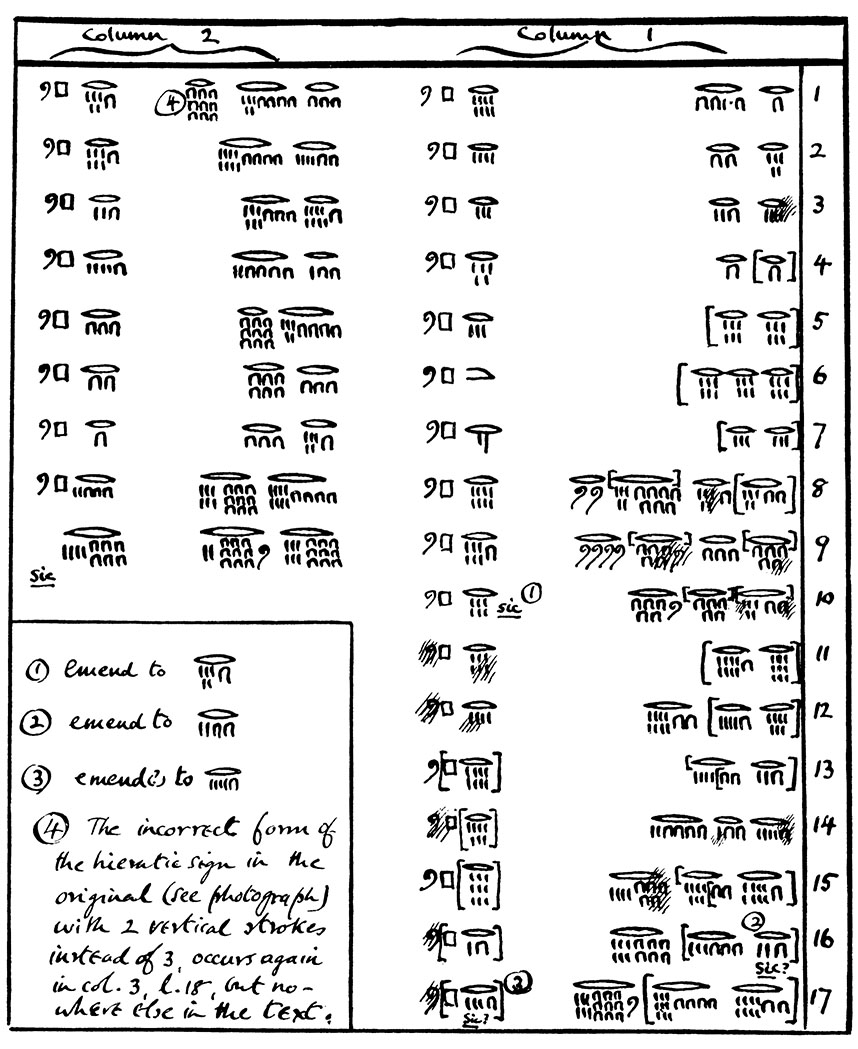
\includegraphics[width=\textwidth]{gfx/EMLRschematic}
  \caption[Schematic of columns 1 and 2 of the Egyptian Mathematical Leather Roll.]
  {Schematic of columns 1 and 2 of the Egyptian Mathematical Leather Roll. Columns 3 and 4 are duplicates of columns 1 and 2. For example, row 1 of column 1 translates to $\displaystyle \frac{1}{10}\frac{1}{40} \quad\quad \frac{1}{8}$ in modern fraction notation where addition is implied. Figure \ref{fig:EMLR} is a photograph of the table outlined here. From \citet{Glanville27} which is accompanied by a translation of the hieroglyphics.}
  \label{fig:EMLRschematic}
\end{figure}

The Egyptian Mathematical Leather Roll, as well as the more famous and extensive Rhine Mathematical Papyrus, were brought to the British Museum in 1864, however it took decades before archaeologists knew how to treat the leather to prevent its disintegration upon unrolling it. \citet{Scott27} provides details of this process and claim that, ``the dissemination of the knowledge of the chemical treatment of the leather, is of greater value than the publication of the contents inscribed on it'' upon discovery of what he considered to be a rather mundane table.

An even more impressive lookup table is found in the extensive Rhind Mathematical Papyrus, which (seemingly) methodologically expresses the fractions $2/n$ for odd $n \in \lbrace 3, 5, \dots, 101 \rbrace$ as the sum of 2--4 unit fractions! We would have chosen to present photographs of the papyrus had the figures of \citep{Glanville27} not been of such high clarity. \citet{Gillings82} reports extensively on this $2/n$ table and the several dozen problems posed and solved on the papyrus, making extensive use of the table. The same table, verbatim, has found to be in use by scribes more than a millennium after its creation suggesting that it was of great utility. To this day, scholars argue about exactly how the scribes knew to construct the table and what methods they used \citep{Gillings74, Abdulaziz08}.

Maybe it is not so surprising that our first approach is to use a lookup table, after all many others have done the same.\footnotemark

\footnotetext{\citet{Neugebauer45} reports on mathematical cuneiform texts used by the ancient Babylonians during similar time periods as well. Other lookup tables of historical importance include a 98-column Roman multiplication table from 493 A.D. \citep{Maher01} and an ancient Indian sine table circa 499 C.E. \citep{Hayashi97}.}

% Of course since then lookup tables have found an enormous number of uses in computer science. Arrays are ubiquitous objects in procedural programming languages and so is the more general dictionary object, especially in Python. Sine tables are still stored in calculators for quick trigonometric computations using the CORDIC algorithm and 3D lookup tables are used in image processing to store color maps. In each case the speed offered by a lookup table once it has been generated is the main reason for their use.

\section{Implementation}

The idea behind using a lookup table is quite simple: many Coulomb explosions are simulated (see section \ref{sec:simulating}) using a wide variety of molecular structures as the initial condition, and the resulting momentum vectors from each simulation are stored. This creates a mapping from molecular structures to momentum vectors. Thus by storing the results from many simulations, we end up with a lookup table. To determine the structure belonging to a certain set of observed momentum vectors, you simply read the table in reverse and search for the momentum vectors that most closely match the observed set.

In our case, we quantify this through the use of the $\ell_2$-norm squared between the sets of vectors
\begin{equation}
\left\|\mathbf{p} - \mathbf{p}'\right\|_2^2
= \sum\limits_{i = 1}^{3N} (p_i - p_i')^2
\end{equation}
for an $N$-atom molecule and where $i$ sums over each momentum component for each atom, \eg $O_x, O_y, \dots, S_y, S_z$ for the \ch{OCS} molecule. We may sometimes refer to as the \emph{objective function} and its value as the \emph{absolute error}.

% TODO: Why the L^2-norm squared?

Each molecular geometry and its corresponding post-explosion momentum vectors can be stored in a single row consisting of $9$ entries, $3$ to describe the molecular geometry of a triatomic molecule and $6$ to describe the momentum vectors. While only $3$ scalars are enough to describe the momentum vectors produced by a simulated Coulomb explosion (the last momentum vector can be calculated from the others using conservation of momentum, see section \ref{sec:conventions}), we store all $6$. This is to allow for comparison with real momentum data where ignoring some component measurements may skew the reconstruction, especially if these specific components happened to carry a large uncertainty. We have not tested this approach when only a subset of our measurements are used, however it may provide a powerful dimensionality-reduction measure when reconstructing larger molecules.

A technical detail that is important to mention is the reason for storing and using bond lengths in units of picometers and bond angles in degrees. The bond lengths and angles differ numerically by approximately 12 orders of magnitude in SI units and so this was done to keep the parameters all on the same order of magnitude, mainly to avoid potential numerical instabilities and to make data analysis and plotting more convenient. This becomes especially important for the optimization approach we take in chapter \ref{ch:optimization} where derivatives and Jacobian matrices need to be calculated. Equivalently, we could have chosen angstroms (\SI{}{\angstrom}) and radians.

A cursory argument in favor of the lookup table would suggest that this approach is simple to implement, fast, and precise as the time-consuming task of simulating many geometries is done only once then stored. Searching through the lookup table to find a match takes linear time $\mathcal{O}(n)$ where $n$ is the number of table entries,\footnotemark~ and the precision is set when simulating the many geometries ($\SI{0.05}{\angstrom}$ and $\SI{0.25}{\angstrom}$ in our case). Big-$\mathcal{O}$ notation is used to refer to the asymptotic behavior of an algorithm's run time or storage space requirements. Even issue we can foresee is that this approach assumes the true geometry is in the vicinity of the geometry found using the lookup table. This is equivalent to assuming that every local minimum is a global minimum (or that this is a convex optimization problem). % One important and interesting exception is the presence of degenerate geometries (section \ref{ssec:degenerateGeometries}).

\footnotetext{It takes linear time because we must search through every single entry before concluding that we have found the best match. If we could sort our entries in some way then we could perform a binary search instead taking logarithmic time $\mathcal{O}(\log n)$ however that would require distilling each entry to an appropriate scalar, which would differ for each geometry and take linear time to perform anyway.}

Momentum lookup tables can be generated using the \texttt{simulateMomenta.m} function and the lookup table is implemented in the \texttt{lookupGeometry.m} file (see appendix \ref{appx:code} for code listings).

% For these reasons, the lookup table was abandoned rather quickly in favor of a mathematical optimization approach that requires no results to be stored, and is aware of the presence of degenerate solutions. But before abandoning it, it is worth analyzing its disadvantages in some detail to explore the nature of the problem of reconstructing geometries. It may have some future usefulness too and we discuss some potential applications.

\subsection{Computational space complexity} \label{ssec:LTspace}

One of the disadvantages of using a lookup table for this particular problem is the amount of storage space it occupies. As a concrete example, our lookup table for \ch{OCS} contained geometries spanning a cube in phase space ($\SI{0.50}{\angstrom} \le r_\mathrm{CO}, r_\mathrm{CS} \le \SI{5.00}{\angstrom}$, $\SI{140}{\degree} \le \theta_\mathrm{OCS} \le \SI{180}{\angstrom}$) that we believe should contain all physically realizable geometries. Individual geometries spanned the discrete ranges $r_\mathrm{CO}, r_\mathrm{CS} \in [0.50, 0.55, \dots, 4.95, 5.00] \SI{}{\angstrom}$ and $\theta_\mathrm{OCS} \in [140.00\degree$, $140.25\degree$, $\dots$, $179.75\degree$, $180.00\degree]$ giving a precision of \SI{0.05}{\angstrom} for the bond lengths and \SI{0.25}{\degree} for the bond angle. This gives us a lookup table with $91 \times 91 \times 161 = 1,333,241$ entries. Since each entry contains $9$ 64-bit floating-point numbers, it requires $9 \times \SI{8}{\byte} = \SI{72}{\byte}$ to store each entry.\footnotemark~ To store the entire table, that is $1,333,241 \times \SI{72}{\byte} = \SI{95.993}{\mega\byte}$. Such a table, if stored in human-readable ASCII such as in a comma-separated value file would take up more space ($\SI{262}{\mega\byte}$) but can be compressed efficiently ($\SI{24}{\mega\byte}$ using 7-zip).

\footnotetext{There are $8$ bits in a byte (\SI{}{\byte}) so a single $64$-bit float would take $8$ bytes to store. MATLAB uses $64$-bit double precision floating point numbers by default but other programming languages may use single precision $32$-bit floating point numbers by default, even when running on a $64$-bit processor.}

For a molecule with $N$ atoms, each entry would require $3N-6$ entries to describe the geometry and $3N-3$ to describe the momentum vectors for a total of $6N-9$ entries per geometry. If $d_i$ denotes the number of values simulated for parameter $i$ (\eg $d_1 = 91$, $d_2 = 91$, and $d_3 = 161$ for our lookup table described above) then the total number of entries will be 
\begin{equation}
\prod\limits_{i=1}^{3N-6} d_i = d_1 \times d_2 \times \dots \times d_{3N-6},
\end{equation}
or simply $d^{3N-6}$ if $d_i = d$ for all $i$ so that we use the same number of simulated values for each parameter. We require \SI{8}{\byte} for each of the $6N-9$ enetries requires to describe each geometry, which we store for $d^{3N-6}$ geometries. Thus the total storage space used up by such a lookup table, in bytes, is 
\begin{equation}
8(6N-9)d^{3N-6}\sim \mathcal{O}(Nd^{N})
\end{equation}
which increases exponentially with an increase in the number of atoms $N$ and follows a power law in the number of simulated values $d$ per parameter. The number of simulated values $d$ required to achieve a certain precision $\epsilon \ll 1$ is $d = (p_\mathrm{max} - p_\mathrm{min})/\epsilon$ where $[p_\mathrm{min}, p_\mathrm{max}]$ is the range of possible parameter values we wish to simulate. So the size of the lookup explodes very quickly with increased precision requirements ($\epsilon \rightarrow 0$) as well, as the desired precision $\epsilon$ is inversely proportional to the step size $d$.

Let us now calculate the size of a higher resolution lookup table and a lookup table for a 4-atom molecule. For example, a lookup table that is five times more precise than ours ($\epsilon_r = \SI{0.01}{\angstrom}$ and $d_r = 451$ for bond lengths, $\epsilon_\theta = \SI{0.05}{\degree}$ and $d_\theta = 801$ for bond angles) takes up $\SI{8}{\byte} \times 9 \times 451^2 \times 801 = \SI{11.7}{\giga\byte}$ of storage space, or $122 \approx 5^3$ times more space. Storing such a table in memory, and thus searching speed which used to only take linear time, starts to become a major concern. Going up to a larger $4$-atom molecule such as acetylene and using the same coarse precision as our lookup table did ($\epsilon_r = \SI{0.05}{\angstrom}$ and $d_r = 91$ for bond lengths, $\epsilon_\theta = \SI{0.25}{\degree}$ and $d_\theta = 161$ for bond angles), a lookup table would take up $\SI{8}{\byte} \times 15 \times 91^3 \times 161^3 = \SI{377}{\tera\byte}$ or almost 4 million times larger, now requiring a distributed database management system; completely overkill to solve a relatively simple problem. It seems that this lookup table approach will not scale at all to larger molecules without massive sacrifices in precision. Plus, using gigabytes to store a lookup table suggests we must seriously look for a method that does not require large amounts of data to reconstruct geometries.

\subsection{Zooming in for more precise reconstructions}

Another immediate disadvantage of such an approach is that you are limited to recovering only the geometries that are included in the table. One way to increase the precision of the lookup table approach without using up additional storage space is to use the table as a coarse first-order approximation. Once a geometry is found using the lookup table, you can dynamically simulate many similar geometries (neighbouring geometries in phase space) on-the-fly which can then be searched for a more precise match. This can be applied iteratively, reducing the volume of phase space searched at each iteration, until a desired precision is reached.

In our case, we chose to increase the precision by a factor of $5$ each iteration so that we search through a cube in phase space with a volume that is $5^3$ times smaller each iteration (in an attempt to precisely locate the local minimum). Each iteration we simulate geometries with $10$ values for each parameter, so $10^3$ geometries in total. We stop after $5$ iterations or after a desired error threshold is reached. Typically an error of $10^{-48}$ gives 1-2 significant figures of precision while an error of $10^{-50}$ gives 2-3 significant figures. This step can be computationally expensive, requiring the additional simulation of thousands of geometries per geometry recovered, however a single simulation takes on the order of $\SI{10}{\ms}$ to complete on a personal laptop so it will complete in a reasonable timeframe and this lets us arbitrarily increase the precision of our reconstruction without using up an exorbitant amount of storage space. It does feel quite wasteful though as it seems that the entire field of mathematical optimization attempts to solve this very problem of finding minima.

One possible improvement is to store these thousands of extra simulations as extra lookup table rows, effectively extending the lookup table. This storing or caching of the results of expensive function calls is termed \emph{memoization}. It may help if the geometries being reconstructed tend to lie close to each other, however in practice the sparsity of reconstructed geometries relative to the resolution of these extra rows results in almost no improvements in performance.

\subsection{Using simulations to test accuracy} \label{ssec:LTaccuracy}
Since we used simulations to test the accuracy of the Nelder-Mead simplex method in section \ref{ssec:simplexFail}, it is only fair that we subject the lookup table to the same analysis. Figure \ref{fig:LookupTableCalibrationPlots} shows the results of this test.

\begin{figure}
  \centering
  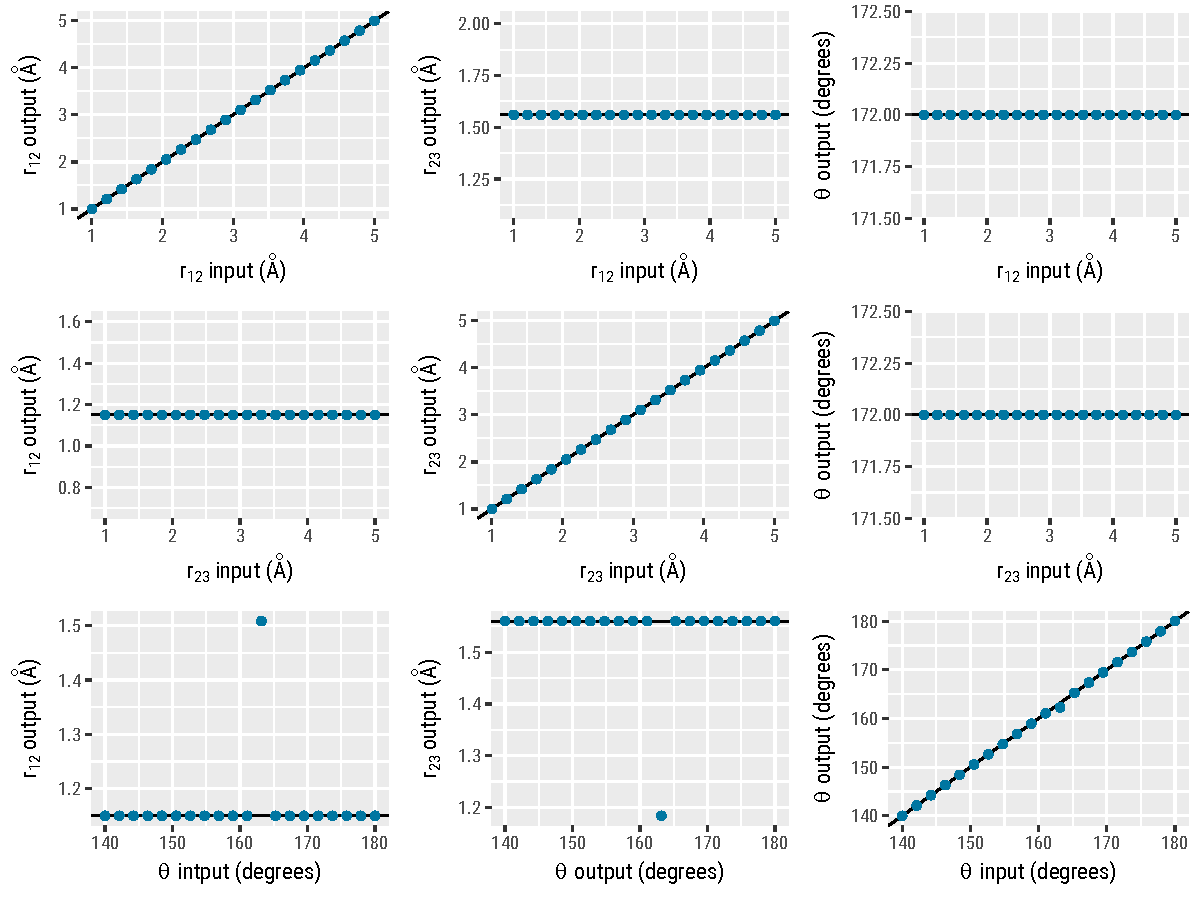
\includegraphics[width=\textwidth]{Plots/LookupTableCalibrationPlots}
  \caption[Testing the Lookup table's ability to reconstruct \ch{OCS} (2,2,2) geometries.]
  {Testing the lookup table's ability to reconstruct \ch{OCS} (2,2,2) geometries by starting with the ground-state geometry of \ch{OCS} and varying each parameter one-by-one. Solid black lines indicate the expected output geometry.}
  \label{fig:LookupTableCalibrationPlots}
\end{figure}

We see that the lookup table is able to reconstruct the vast majority of the geometries quite well, except for a single outlier, suggesting that this approach is already much more reliable as no fine tuning is required at all. It is important to note that we did not simulate geometries that are already contained in the lookup table otherwise the reconstruction is trivial as the table already contains the answer, which is extremely unlikely if we are dealing with experimental data.

\section{Reconstruction of experimental data} \label{sec:LTgeometries}

% With the knowledge that the lookup table can be somewhat trusted, we should use it to reconstruct some real geometries.

We will now attempt to use the lookup table to reconstruct the \ch{OCS} $(2,2,2)$ geometry as an example. Figure \ref{fig:OCS2227fsLTGeometry} shows one such geometry for the Coulomb explosion by a \SI{7}{\femto\s} laser pulse and may form the first frame of a molecular movie.

\begin{figure}
  \centering
  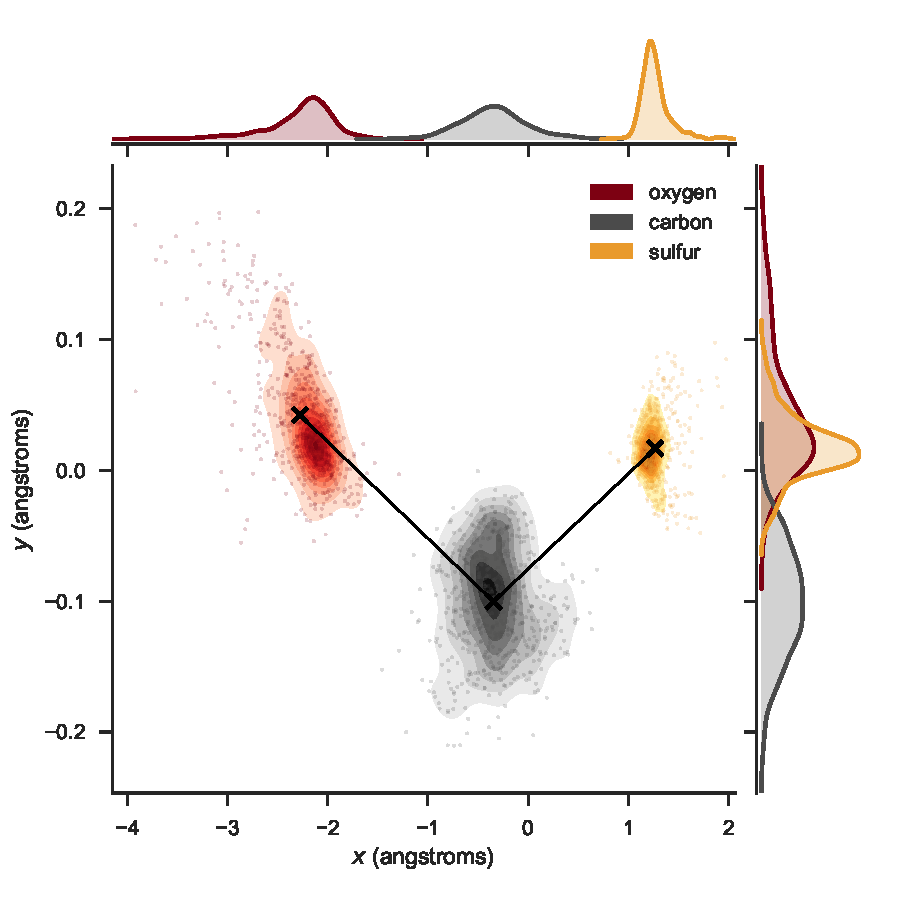
\includegraphics[width=\textwidth]{Plots/OCS2227fsLTGeometry}
  \caption[Scatter plot showing the molecular geometry of \ch{OCS} following Coulomb explosion by a \SI{7}{\fs} laser pulse for the $(2,2,2)$ fragmentation channel.]
  {Scatter plot showing the molecular geometry of \ch{OCS} following Coulomb explosion by a \SI{7}{\fs} laser pulse for the $(2,2,2)$ fragmentation channel. Each geometry is represented by three colored points, one for each atomic fragment; red for oxygen on the left, black for carbon in the center, and yellow for sulfur on the right. The colors were chosen to imitate the CPK coloring convention. Geometries are plotted such that the molecule's center of mass is at the origin to showcase the variance in each atomic fragment's position, and are rotated such that a vertical line bisects the \ch{O-C-S} bond angle. Bivariate kernel density estimates (with a Gaussian kernel), plotted as shaded-in contours, are used to estimate the the probability density of each atomic fragment's position. Solid black lines are drawn between the peaks of each atomic fragment's kernel density estimate to illustrate the \emph{modal geometry} or most likely geometry. Along the top of the plot, marginal distributions show the probability density of each atomic fragment's position along the $x$-axis and the same is done for the $y$-axis along the right. The molecule is almost straight but an aspect ratio of approximately $12:1$ is employed to showcase variability in the $y$-axis.}
  \label{fig:OCS2227fsLTGeometry}
\end{figure}

Here we have plotted the geometries by placing the center of mass at the origin, giving us three probability distributions, one for each atomic fragment which allows us to see the variance in each atomic fragment's position. We could have placed the carbon at the center resulting in just two distributions, one for each of the terminal atoms much like \citet{Brichta07} did in figure \ref{fig:simplexJPhysB} however we felt that this approach provides less information. \cite{Bocharova11}, in figure \ref{fig:simplexPRL}, plot the geometries with a terminal oxygen at a fixed position along the $x$-axis and include a one-dimensional marginal distribution of the oxygen's position along the $x$-axis, which is an improvement but we feel that it still provides less information.  We use the same visualization method as \citet{Legare05structure} (see figure \ref{fig:SO2-232structure}) who revert to a plot like the one by \citet{Bocharova11} in their later work \citep{Legare05dynamics}. The modal geometry is calculated to be $r_\mathrm{CO} = \SI{1.74}{\angstrom}$, $r_\mathrm{CS} = \SI{1.59}{\angstrom}$, $ \theta_\mathrm{OCS} = 172.7\degree$ while the average geometry of $r_\mathrm{CO} = \SI{1.93}{\angstrom}$, $r_\mathrm{CS} = \SI{1.61}{\angstrom}$, $ \theta_\mathrm{OCS} = 171.6\degree$ is slightly larger due to outliers.

An argument could be made for each visualization method, however we will come back the issue of geometry plotting later in chapter \ref{ch:optimization}, where we will look at correlations between bond lengths.

% in the end it probably does not matter how the geometries are plotted. In chapter \ref{ch:optimization} we will see that plotting geometries in this manner alone, while intuitive and satisfying, can be very misleading in that it can be used to hide unphysical data and make it appear agreeable. This is because the ensemble of geometries reconstructed seems to make physical sense while most of the individual geometries reconstructed do not upon further inspection. We do not know much about the individual geometries from such a plot as we do not know which points are correlated with which.

% TODO: Any explanation for this?
The calculated modal and average geometries may appear quite worrying as they suggest a stretching of the \ch{C-O} bond while the \ch{C-S} bond and the bond angle remains close to equilibrium. This is mainly due to ion motion from the molecule's interaction with the laser pulse during the ionization process. % Now, I'm not saying they're right or wrong, just that I don't trust them.

A critical issue worth investigating is quantifying how much uncertainty there is in these reconstructed molecular geometries. This is a complicated problem we will tackle in chapter \ref{ch:uncertainty}.

We can repeat this analysis for the other laser pulse widths (\SIlist{30;60;100;200}{\fs}). In table \ref{table:lookupTableSuccess} we tabulate the number of geometries we were able to successfully reconstruct, which decreases as the pulse length increases indicating a greater difficulty in reconstructing geometries that are further from equilibrium. Or it could indicate a greater difficulty in reconstructing geometries when the atomic fragments had some significant initial momentum. The longer the laser pulse, the more time the molecule has to distort its structure in response to the laser's intense electric field, reducing the validity of the assumption that the molecule begins the Coulomb explosion process in its equilibrium geometry.

To conserve space, the geometry reconstructions for Coulomb explosion by \SIlist{30;60;100;200}{\fs} laser pulses are provided in appendix \ref{appx:supplementaryFigures} (figures \ref{fig:OCS22230fsLTGeometry}--\ref{fig:OCS222200fsLTGeometry}).

\begin{table}
  \myfloatalign
  \centering
  \begin{tabularx}{0.875\textwidth}{cccc}
    \toprule
    Pulse width (\SI{}{\fs}) & Geometries & Reconstructions & Success \\
    \midrule
    7 & 795 & 584 & 73\% \\
    30 & 1000 & 518 & 52\% \\
    60 & 358 & 154 & 43\% \\
    100 & 531 & 226 & 43\% \\
    200 & 500 & 190 & 38\% \\
    \bottomrule
  \end{tabularx}
  \caption[Statistics for geometry reconstruction by lookup table.]
  {Statistics for geometry reconstruction by lookup table.}
  \label{table:lookupTableSuccess}
\end{table}

Of particular interest might be the average and modal (most likely) geometries recovered, which we tabulate in table \ref{table:lookupTableGeometries}.

\begin{table}
  \myfloatalign
  \centering
  \begin{tabularx}{0.9\textwidth}{ccccccc}
    \toprule
    Pulse & \multicolumn{3}{c}{Modal geometry} & \multicolumn{3}{c}{Average geometry} \\
    length (fs) & $r_\mathrm{CO}$ & $r_\mathrm{CS}$ & $\theta_\mathrm{OCS}$ & $r_\mathrm{CO}$ & $r_\mathrm{CS}$ & $\theta_\mathrm{OCS}$ \\
    \midrule
    (Equilibrium) & 1.16 & 1.56 & 172 & 1.16 & 1.56 & 172 \\
    7 & 1.74 & 1.59 & 173 & 1.93 & 1.61 & 172 \\
    30 & 2.34 & 1.74 & 172 & 2.50 & 2.04 & 170 \\
    60 & 2.43 & 1.96 & 171 & 2.56 & 2.16 & 170 \\
    100 & 2.52 & 2.16 & 171 & 2.72 & 2.46 & 169 \\
    200 & 3.17 & 2.22 & 171 & 3.10 & 2.72 & 163 \\
    \bottomrule
  \end{tabularx}
  \caption[Average and modal geometries reconstructed using a lookup table.]
  {Average and modal geometries reconstructed using a lookup table. Bond lengths are given in angstroms (\SI{1}{\angstrom} = \SI{e-10}{\m}) and bond angles in degrees.}
  \label{table:lookupTableGeometries}
\end{table}

% Probability distributions for the atomic positions in the $xy$-plane and along both the $x$- and $y$-axes in figure \ref{fig:OCS2227fsLTGeometry} are estimated using kernel density estimates (KDE's) which may be thought of as a smoothed histogram that integrates to one (like a probability distribution). 

\section{Degenerate molecular geometries} \label{sec:degenerateGeometries}
In chapter \ref{ch:introduction} we hinted at the fact that due to the ill-posed nature of the geometry reconstruction inverse problem, multiple solutions may be possible. While investigating the reconstructed geometries, this feature surprisingly did appear for the \ch{OCS} molecule and the lookup table can help provide some insight into these multiple solutions, which we will call \emph{degenerate geometries}.

Figure \ref{fig:rainbow} shows an example of two degenerate geometries that both produce the same set of momentum vectors after a Coulomb explosion, $\mathbf{p}_O = (0.398, -1.75, 0) \times \SI[per-mode=symbol]{e-20}{\kilogram\metre\per\second}$, $\mathbf{p}_C = (0.853, 0, 0) \times \SI[per-mode=symbol]{e-20}{\kilogram\metre\per\second}$, and $\mathbf{p}_S = (-1.25, 1.75, 0) \times \SI[per-mode=symbol]{e-20}{\kilogram\metre\per\second}$ (described in our convention).
\begin{figure}
  \centering
  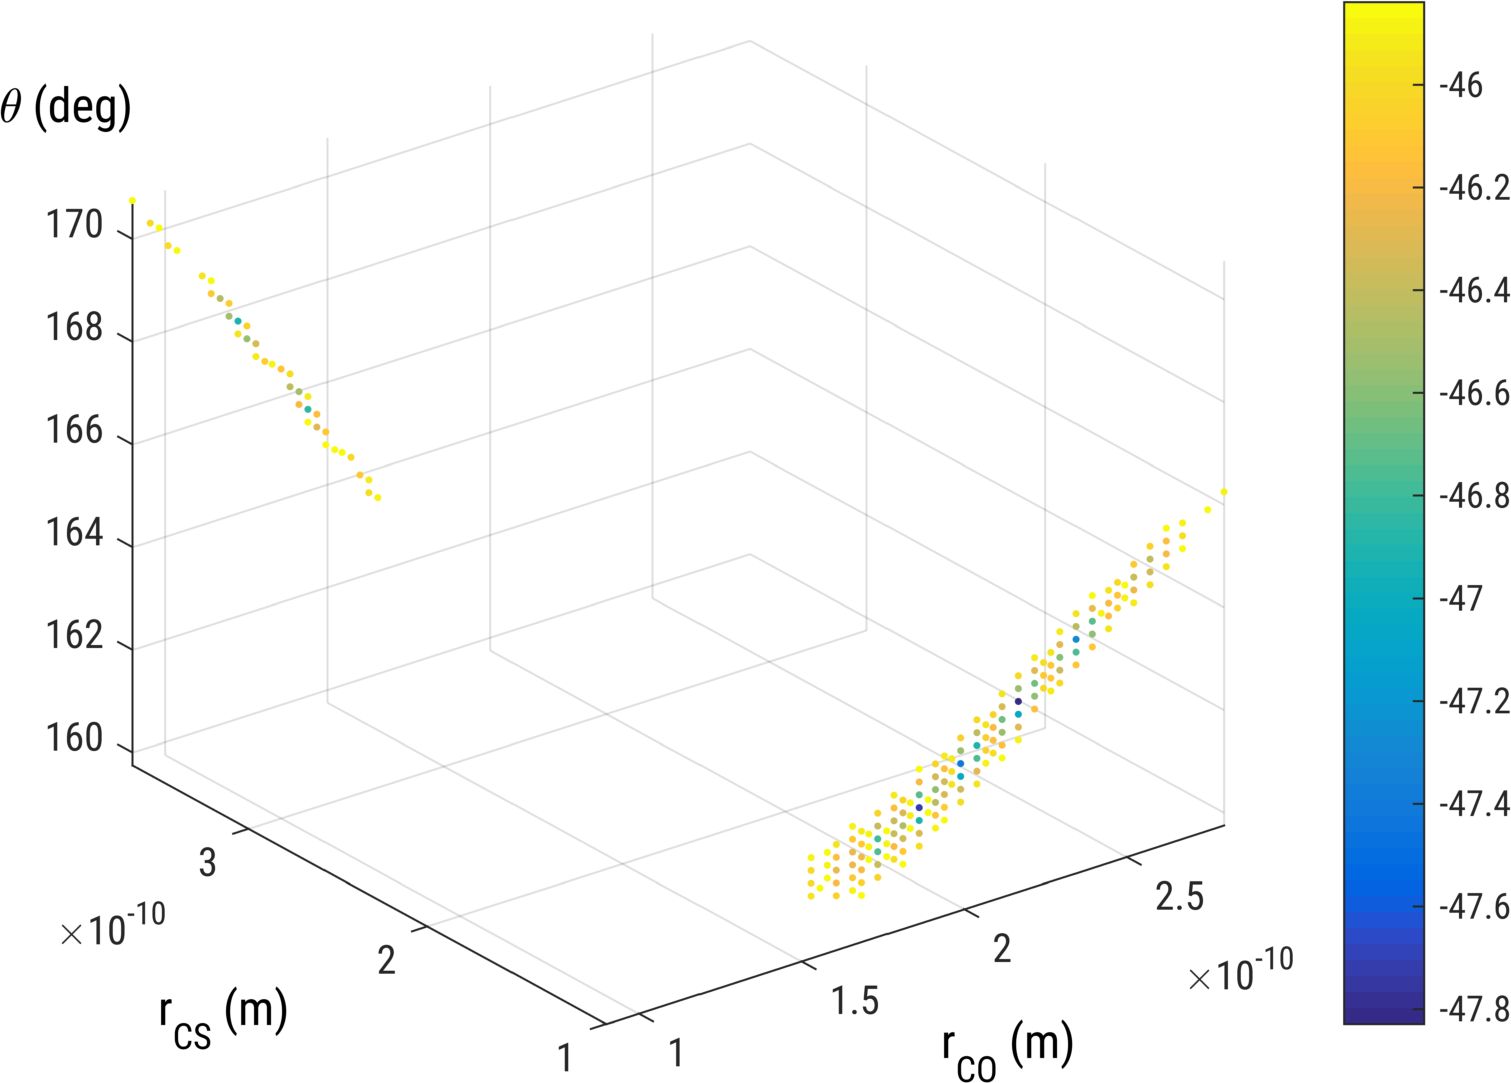
\includegraphics[width=\textwidth]{Plots/rainbow}
  \caption[3D scatter plot in phase space of the $200$ best geometries matching a particular set of measured momentum vectors, showing the existence of two degenerate geometries.]
  {3D scatter plot in phase space of the $200$ best geometries matching a particular set of measured momentum vectors, showing the existence of two degenerate geometries. Each point is colored according to the base-$10$ logarithm of the absolute error ($2$-norm) squared between the measured momentum vectors and the momentum vectors resulting from Coulomb exploding the geometry corresponding to that data point.}
  \label{fig:rainbow}
\end{figure}

More specifically, it is a $3$D scatter plot in phase space of the $200$ best geometries matching this particular set of measured momentum vectors. Each point is colored according to the base-$10$ logarithm of the absolute error ($2$-norm) squared between the measured momentum vectors and the momentum vectors resulting from Coulomb exploding the geometry corresponding to that data point. So the darkest purple corresponds to an error of just under $10^{-47.8}$. The $200$ best geometries are clustered into two separate regions, indicating that the particular set of measured momentum vectors mentioned above could have resulted from the Coulomb explosion of two very different molecular geometries, one where the \ch{C-O} bond is more stretched, and another where the \ch{C-S} bond is more stretched and the molecule is less bent. Interestingly, the points do not seem to form balls or blobs in phase space, but rather possess elongated and angled rod-like distributions. The region with the stretched \ch{C-O} bond seems to have more points but this does not suggest that this geometry is more likely. Rather, it may suggest that it is easier to converge to, or that it may have a larger \emph{basin of attraction}. We see that there are many yellow data points (relatively high error) surrounding one or two purple points (relatively low error) for each region indeed showing the low-resolution nature of our lookup table. This same information may be plotted using $2$D color mapped volumetric slices or contour slices which may even be animated to provide a visual scan through the full phase space volume. However due to the angled distribution formed by the spatial sets and the significance of only one or two data points, it becomes very difficult to visually locate the local minima even with angled slices. Another visualization method may be to use convex hulls or alpha shapes which will also allow us to assign each region a shape and volume (see section \ref{ssec:convexAlpha}).

In figure \ref{fig:DegenerateGeometryTrajectories} we take these two degenerate geometries, Coulomb explode them, and plot their trajectories to show that even though they show slightly different dynamics, both simulations result in the exact same momentum vectors (and kinetic energy) being measured.

\begin{figure}
  \centering
  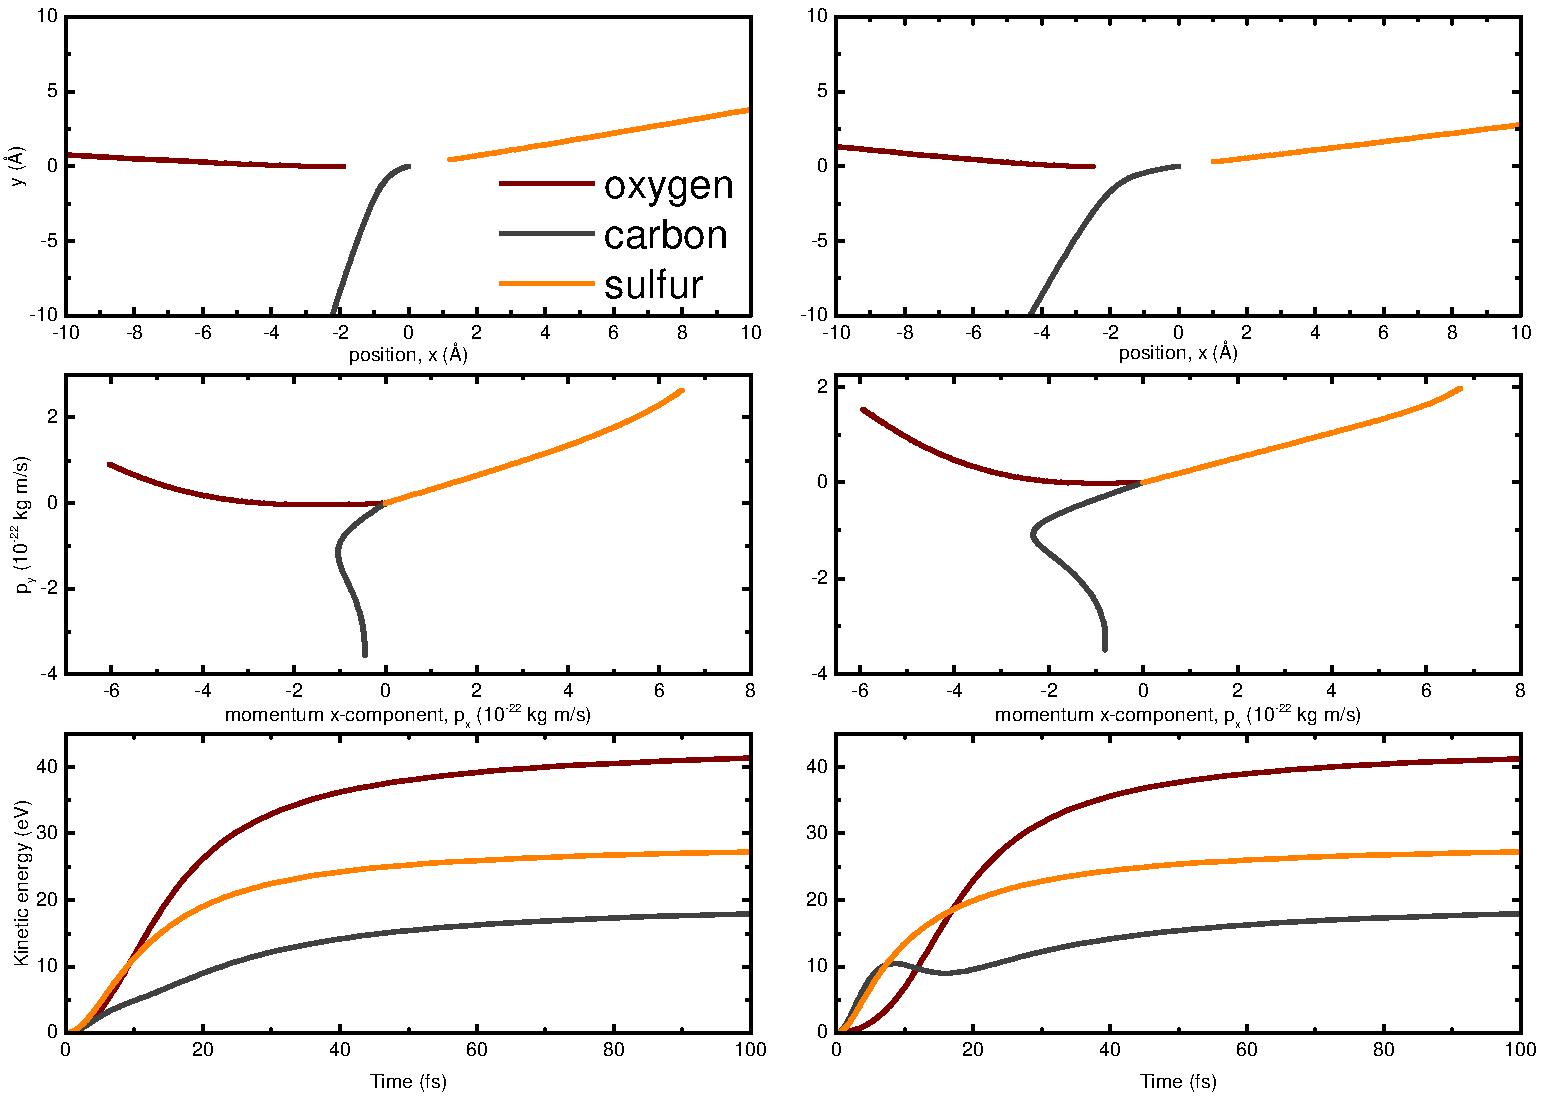
\includegraphics[width=\textwidth]{Plots/DegenerateGeometryTrajectories.pdf}
  \caption[Atomic trajectories in position and momentum-space, and kinetic energy, of two degenerate molecular geometries undergoing a Coulomb explosion.]
  {Atomic trajectories in position and momentum-space, and kinetic energy, for the oxygen, carbon, and sulfur atoms of two degenerate \ch{OCS} molecular geometries in the $(2,2,2)$ charge state undergoing a Coulomb explosion staring from rest.}
  \label{fig:DegenerateGeometryTrajectories}
\end{figure}

The plots on the left correspond to an \ch{OCS} molecule with $r_\textrm{CO} = \SI{1.8949}{\angstrom}$, $r_\textrm{CS} = \SI{1.2990}{\angstrom}$, and $\theta_\mathrm{OCO} = \SI{160.601}{\degree}$ while the plots on the right correspond to an \ch{OCS} molecule with $r_\textrm{CO} = \SI{2.486}{\angstrom}$, $r_\textrm{CS} = \SI{1.0755}{\angstrom}$, and $\theta_\mathrm{OCO} = \SI{164.568}{\degree}$. Triatomic molecules explode in a plane so their momentum vectors can be plotted in the $p_xp_y$-plane although the atomic fragments will possess some momentum in the $z$-direction due to the presence of the constant electric field, it will not deviate from equation \eqref{eq:CEImomenta} and is irrelevant for these simulated Coulomb explosions. The molecular geometries are quite different yet when they undergo a Coulomb explosion, they produce the exact same set of momentum vectors once rotated into our convention (see section \ref{sec:conventions}). By that we mean that we can make the absolute error (or $2$-norm) between the two sets of momentum vectors arbitrarily small with increased precision in describing the geometries. We see that the molecular dynamics are a little different yet in both cases, all three atoms emerge with the exact same kinetic energy. These two geometries were found by searching through the entire lookup table for the geometries best matching a particular set of measured momentum vectors (see figure \ref{fig:rainbow}). The lookup table actually does not give us enough precision to recover these geometries to several decimal places so we used the lookup table to find a measurement corresponding to two degenerate geometries, and then used the optimization method from chapter \ref{ch:optimization} to actually recover the geometries with much higher precision.

The high precision to which we were able to recover the two degenerate geometries suggests that presence of degenerate geometries corresponds to the existence of multiple global minima. This suggests the use of a method that can locate multiple minima, which we will employ in the next chapter.

\section{Conclusions}
\emph{Geometries may be reconstructed using a lookup table}---We find this approach more reliable and robust that the Nelder-Mead simplex method approach employed by \citet{Brichta09}, and it has provided us with some additional insight into the problem of reconstructing geometries especially regarding the existence of degenerate geometries. This makes the lookup table potentially useful for future investigations and reconstructions of triatomic molecules. However, it seems that it will not scale to molecules containing more than $3$ atoms, motivating the need for another method.

\subsection{Lessons learnt}
% \emph{Degenerate geometries exist}---An unexpected result of \\

\noindent
\emph{Inability to precisely reconstruct geometries}---Using just the lookup table itself, you are limited to recovering molecular geometries contained in the lookup table and nothing in between, severely limiting the resolution of reconstructed geometrie. \\

\noindent
\emph{Inability to differentiate between global and local minima}---The lookup table cannot choose between two degenerate geometries and due to it's low resolution it cannot distinguish between global and local minima. It may be easily modified to report on multiple solutions but doing so may be computationally expensive. A more sophisticated approach should be sought first. \\

\noindent
\emph{Inability to scale to larger molecules}---As discussed in section \ref{ssec:LTspace}, trying to use the lookup table to reconstruct molecules containing even as little as 4 atoms requires prohibitive amounts of storage space ($\SI{>100}{\tera\byte}$) to store the lookup table. This may be circumvented by fixing some molecular parameters, such as maybe the \ch{C+C} triple bond length in acetylene, if they vary very little and are not of interest. However, this fix only reduces the dimensionality by one so it is unlikely to be an overall solution.

\subsection{Future applications for the lookup table}

\emph{Finding an initial or first-order solution or initial guess}---As the lookup table may quickly find coarse-grained geometries, the recovered geometry may be used as an initial guess or first-order solution for another algorithm. \\

\noindent
\emph{Visualizing the reconstruction problem for a specific set of momentum vectors}---Such a plot would assign a scalar error value to every point in phase space, allowing us to quickly visualize the objective function (as done in figure \ref{fig:rainbow} but for all the geometries, not just the best $200$). This would visualize the location of degenerate geometries and provide some insight into the nature of the geometry reconstruction problem. For example, if it is smooth and convex with a single global minimum, it would suggest that geometry reconstruction in that particular case is computationally easy. However, a jagged and discontinuous function with multiple minima and saddle points would suggest that geometry reconstruction is much more difficult. For triatomic molecules the $3$-dimensional space may be visualized using colormapped volumetric slices or contour slices. Unfortunately this becomes unfeasible for larger molecules due both the size of the lookup table and the difficulty of visualizing an $n$-dimensional scalar function ($n>3$). Instead of generating a lookup table for larger molecules, Coulomb explosions can be simulated for every geometry of interest, if the resolution is reduced. Fixing certain parameters would reduce the dimensionality of the objective function, allowing $2$-dimensional slices of it to be easily visualized. Or one could look towards methods of visualizing high-dimensional scalar functions. \\

\noindent
\emph{Finding degenerate regions of phase space quickly}---At least for triatomic molecules, where generating and storing a lookup table is feasible, it may be quickly searched to determine whether a set of measured momentum vectors correspond to just one geometry, or multiple degenerate geometries.
